\subsection{\gls{crna} quantification}
\label{sec:crna_quantification}

While all \gls{bsj} detection tools quantify the number of reads
supporting each \gls{bsj}, there are several tools that focus on the
quantification of \glspl{crna} based on previously detected \glspl{bsj}.
nf-core/circrna offers two such tools: CIRIquant and
psirc-quant.

\subsubsection{CIRIquant}
\label{sec:ciriquant}
CIRIquant extends the CIRI (\Gls{crna} Identifier) framework, focusing on
accurate \gls{crna} quantification by re-aligning \gls{bsj} reads to a
pseudo-reference sequence.
Although it natively utilizes CIRI2 for \gls{bsj} detection, it can also
process \glspl{bsj} identified by other tools\supercite{zhang_accurate_2020}.
For each \gls{bsj}, CIRIquant constructs a pseudo \gls{crna} reference by
concatenating two copies of the sequence between the \gls{bsj} start and end
positions.
By comparing alignments to both the reference genome and the pseudo-reference
sequence, CIRIquant calculates the fraction of reads utilizing the \gls{bsj}
among those that span at least one of its
boundaries\supercite{zhang_accurate_2020}.
The output provided by CIRIquant is essentially the CPM (counts per million) of
reads supporting each \gls{bsj}, normalized by the total number of mapped reads
in the sample.

\subsubsection{psirc}
\label{sec:psirc}
As illustrated in \cref{fig:psirc_workflow}, psirc operates in two main phases:
first, the identification of \gls{bsj} and inference of full-length isoforms
(FLI); and second, the quantification of expression levels for the detected
isoforms\supercite{yu_quantifying_2021}.

\begin{figure}[ht] \centering

    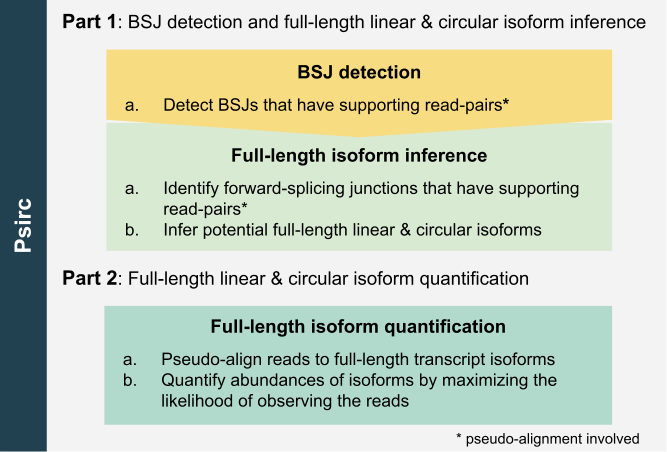
\includegraphics[width=0.5\textwidth]{chapters/3_materials_and_methods/figures/psirc_pipeline.png}
    \caption{psirc-workflow} \label{fig:psirc_workflow} \end{figure}

The initial phase of the workflow functions similarly to the implementation
described in \cref{sec:ciriquant}, with the added step of full-length isoform
inference.
However, this step requires paired-end sequencing data, which is not available
in this thesis.
While psirc's \gls{bsj} detection can be substituted with other tools, the FLI
inference step is more challenging to replace.
Previous studies have attempted to address this by using information from the
linear transcriptome to retain only exonic regions within the \gls{bsj} limits
\supercite{hoffmann_circrna-sponging_2023}.
If no exonic regions are present, the entire sequence is retained.
In contrast, the nf-core/circrna pipeline takes a different approach, retaining
the entire sequence within the \gls{bsj} boundaries, regardless of exonic
region presence.
This method avoids assumptions about the internal structure of the \gls{crna}.

For the quantification phase, psirc requires a combined transcriptome FASTA
file containing both linear and circular transcripts.
Psirc constructs a Transcript de Bruijn Graph (T-DBG) from this combined
transcriptome and utilizes Kallisto to jointly quantify the expression levels
of both transcript types\supercite{yu_quantifying_2021}.
This approach enables a direct comparison between linear and circular isoforms,
potentially offering deeper insights into the regulatory roles of \glspl{crna}
in gene expression.
Notably, psirc does not explicitly differentiate between reads spanning the
\gls{bsj} and those fully contained within it; instead, it relies on Kallisto's
likelihood maximization to distinguish between linear and circular
isoforms\supercite{yu_quantifying_2021}.
